% Importado desde: 2026-03-28_Seleccion_del_Subsector_Efectivo_en_3D.tex
\chapter{Derivacion Pedagogica: --- seleccion del subsector efectivo en una dinamica discreta \(3D\)}
\label{ch:subsector-efectivo-3d}






% verified-by: validators/wilson_subsector.py::test_massless_at_zero
% verified-by: validators/wilson_subsector.py::test_doubler_mass_at_pi
% verified-by: validators/wilson_subsector.py::test_linearization_is_dirac
% verified-by: validators/wilson_subsector.py::test_squared_at_corners

\section{Objetivo}
Despues de entender:
\begin{enumerate}[label=\arabic*.]
    \item como aparece un sector tipo Weyl o Dirac al linealizar;
    \item como se organizan las matrices gamma y los generadores de Lorentz;
    \item y por que Nielsen--Ninomiya obliga a contar todos los nodos,
\end{enumerate}
la pregunta mas delicada del proyecto pasa a ser esta:
\begin{displayquote}
\textbf{como se dise\~na una dinamica discreta concreta para que exista un subsector de baja energia bien controlado, relativista y distinguible del resto de los dobladores?}
\end{displayquote}

Este capitulo responde esa pregunta paso a paso usando el modelo de red mas pedagogico para hacerlo:
\begin{equation}
\text{el Hamiltoniano de Wilson--Dirac en \(3D\)}.
\end{equation}

La razon para elegirlo es muy simple:
\begin{enumerate}[label=\arabic*.]
    \item usa exactamente la algebra de Dirac que ya construimos;
    \item vive en una red discreta y por tanto ve el problema global de doblamiento;
    \item incorpora de forma controlada un mecanismo para hacer pesados a los dobladores;
    \item permite ver con formulas explicitas cuando un solo subsector queda ligero.
\end{enumerate}

\section{La idea fisica antes de las cuentas}
El problema global de la discretizacion ingenua es que varios nodos de Dirac o Weyl aparecen al mismo tiempo. Si todos quedan con energias comparables, no existe un solo sector relativista limpio: existen varios, mezclados en la misma ventana de energia.

La estrategia correcta es entonces:
\begin{enumerate}[label=\arabic*.]
    \item mantener ligero el sector que queremos estudiar;
    \item empujar los demas a energias mucho mas altas;
    \item trabajar despues en una ventana de energia donde esos sectores pesados no se exciten.
\end{enumerate}

En lenguaje efectivo, lo que buscamos es una jerarquia de escalas:
\begin{equation}
\abs{E} \ll \Delta_{\text{heavy}},
\end{equation}
donde \(\Delta_{\text{heavy}}\) es la masa o gap minimo de los dobladores no deseados.

\begin{figure}[h!]
\centering
\begin{tikzpicture}[
    box/.style={draw, rounded corners, thick, align=center, minimum width=3.8cm, minimum height=1.3cm},
    arr/.style={-{Latex[length=3mm]}, thick}
]
\node[box, fill=blue!7] (a) at (0,0) {red discreta\\muchos nodos};
\node[box, fill=yellow!10] (b) at (4.8,0) {introducir termino\\de Wilson};
\node[box, fill=green!7] (c) at (9.6,0) {un sector ligero\\otros pesados};
\node[box, fill=red!7] (d) at (14.4,0) {teoria efectiva\\relativista controlada};
\draw[arr] (a) -- (b);
\draw[arr] (b) -- (c);
\draw[arr] (c) -- (d);
\end{tikzpicture}
\caption{La logica completa del paso que queremos justificar.}
\end{figure}

\section{Por que elegimos el modelo de Wilson--Dirac}
\subsection{La forma del Hamiltoniano}
Tomamos
\begin{equation}
H(\bm{k})=
\frac{v}{a}\sum_{i=1}^3 \sin(k_i a)\,\alpha_i
+
M(\bm{k})\,\beta,
\label{c14:eq:wilsondirac}
\end{equation}
donde
\begin{equation}
M(\bm{k}) = m + r\sum_{i=1}^3 \left(1-\cos(k_i a)\right).
\label{c14:eq:massfunction}
\end{equation}

Aqui:
\begin{enumerate}[label=\arabic*.]
    \item \(a\) es el espaciado de red;
    \item \(v\) fija la velocidad efectiva;
    \item \(m\) es la masa bare o masa de referencia;
    \item \(r\) controla el termino de Wilson;
    \item \(\alpha_i,\beta\) satisfacen la algebra de Dirac
    \[
    \{\alpha_i,\alpha_j\}=2\delta_{ij}\mathbb{I}_4,
    \qquad
    \{\alpha_i,\beta\}=0,
    \qquad
    \beta^2=\mathbb{I}_4.
    \]
\end{enumerate}

Una realizacion concreta, compatible con nuestros capitulos anteriores, es
\begin{equation}
\alpha_i=\tau_z\otimes \sigma_i,
\qquad
\beta=\tau_x\otimes \mathbb{I}_2.
\end{equation}

\subsection{Por que esta eleccion es la correcta}
Cada parte del Hamiltoniano tiene una funcion precisa:
\begin{enumerate}[label=\arabic*.]
    \item \(\sin(k_i a)\alpha_i\) reproduce el termino lineal tipo Dirac cerca de \(\bm{k}=0\);
    \item \(m\beta\) controla la masa del sector central;
    \item el termino con \(r(1-\cos k_i a)\) casi no afecta al sector central a primer orden, pero si afecta mucho a los nodos situados cerca de los bordes de la zona de Brillouin.
\end{enumerate}

Esa asimetria es exactamente lo que necesitabamos.

\section{El espectro completo}
Como \(\alpha_i\) anticomutan entre si y con \(\beta\), el cuadrado del Hamiltoniano es escalar:
\begin{equation}
H(\bm{k})^2=
\left[
\frac{v^2}{a^2}\sum_{i=1}^3 \sin^2(k_i a)+M(\bm{k})^2
\right]\mathbb{I}_4.
\end{equation}

Por tanto el espectro es
\begin{equation}
E(\bm{k})=
\pm
\sqrt{
\frac{v^2}{a^2}\sum_{i=1}^3 \sin^2(k_i a)+M(\bm{k})^2
}.
\label{c14:eq:spec}
\end{equation}

La informacion crucial sobre los nodos y los gaps esta toda contenida en \(M(\bm{k})\).

\section{Los ocho puntos especiales de la zona de Brillouin}
Los puntos de referencia naturales son
\begin{equation}
\bm{K}^{(n_x n_y n_z)}=
\left(
\frac{n_x\pi}{a},
\frac{n_y\pi}{a},
\frac{n_z\pi}{a}
\right),
\qquad
n_i\in\{0,1\}.
\label{c14:eq:TRIM}
\end{equation}

En esos puntos:
\begin{equation}
\sin(K_i a)=0,
\qquad
\cos(K_i a)=(-1)^{n_i}.
\end{equation}
Entonces la masa efectiva se vuelve
\begin{equation}
M_n = m + 2rN_n,
\qquad
N_n=n_x+n_y+n_z.
\label{c14:eq:Mn}
\end{equation}

Esto ya resume casi toda la fisica del control de dobladores. Los ocho nodos no son ya equivalentes: se agrupan por el numero \(N_n\) de componentes que valen \(\pi/a\).

\begin{center}
\begin{tabular}{c c c}
\toprule
\(N_n\) & multiplicidad & masa efectiva \\
\midrule
0 & 1 & \(m\) \\
1 & 3 & \(m+2r\) \\
2 & 3 & \(m+4r\) \\
3 & 1 & \(m+6r\) \\
\bottomrule
\end{tabular}
\end{center}

\section{Linealizacion paso a paso alrededor de cada punto}
Sea
\begin{equation}
\bm{k}=\bm{K}^{(n)}+\bm{q},
\qquad
\abs{\bm{q}}a\ll 1.
\end{equation}

\subsection{Termino cinetico}
Tenemos
\begin{equation}
\sin(K_i a + q_i a)=(-1)^{n_i}\sin(q_i a)\simeq (-1)^{n_i}q_i a.
\end{equation}
Asi,
\begin{equation}
\frac{v}{a}\sin(k_i a)\alpha_i
\simeq
v(-1)^{n_i}q_i\alpha_i.
\end{equation}

\subsection{Termino de Wilson}
Ahora
\begin{align}
1-\cos(K_i a+q_i a)
&=
1-\cos(K_i a)\cos(q_i a)+\sin(K_i a)\sin(q_i a)
\\
&=
1-(-1)^{n_i}\cos(q_i a).
\end{align}
Como
\begin{equation}
\cos(q_i a)\simeq 1-\frac{(q_i a)^2}{2},
\end{equation}
se obtiene:
\begin{enumerate}[label=\arabic*.]
    \item si \(n_i=0\): \(1-\cos(K_i a+q_i a)\simeq \frac{(q_i a)^2}{2}\);
    \item si \(n_i=1\): \(1-\cos(K_i a+q_i a)\simeq 2-\frac{(q_i a)^2}{2}\).
\end{enumerate}

Por tanto, a primer orden en \(\bm{q}\), el termino de Wilson no cambia la parte lineal: solo fija una masa distinta en cada punto.

\subsection{Hamiltoniano efectivo}
Juntando ambas partes, cerca de \(\bm{K}^{(n)}\) obtenemos
\begin{equation}
H^{(n)}_{\text{eff}}(\bm{q})
\simeq
v\sum_{i=1}^3 (-1)^{n_i}q_i\alpha_i
+
M_n\beta,
\label{c14:eq:Heffn}
\end{equation}
con \(M_n\) dado por \eqref{c14:eq:Mn}.

Este es el punto clave:
\begin{displayquote}
\textbf{el termino de Wilson no elimina la estructura tipo Dirac local; lo que hace es asignar masas diferentes a los distintos dobladores.}
\end{displayquote}

\section{Como se selecciona un solo subsector ligero}
Queremos que el sector alrededor de \(\bm{k}=0\) sea ligero, y los demas pesados.

\subsection{Sector central}
Para \((n_x,n_y,n_z)=(0,0,0)\) tenemos
\begin{equation}
M_{000}=m.
\end{equation}
Asi que, si \(\abs{m}\) es peque\~na, ese sector queda ligero.

\subsection{Sectores dobladores}
Los otros sectores tienen masas
\begin{equation}
m+2r,\qquad m+4r,\qquad m+6r.
\end{equation}
Si elegimos \(r>0\) y
\begin{equation}
\abs{m}\ll 2r,
\label{c14:eq:window}
\end{equation}
entonces:
\begin{enumerate}[label=\arabic*.]
    \item el sector central tiene masa peque\~na;
    \item los sectores con \(N=1\) tienen masa del orden \(2r\);
    \item los sectores con \(N=2\) tienen masa del orden \(4r\);
    \item el sector con \(N=3\) tiene masa del orden \(6r\).
\end{enumerate}

La jerarquia de escalas queda entonces bien definida:
\begin{equation}
\Delta_{\text{heavy}}
=
\min\left\{
\abs{m+2r},
\abs{m+4r},
\abs{m+6r}
\right\}
\simeq 2r
\quad
\text{si } \abs{m}\ll 2r.
\label{c14:eq:gapheavy}
\end{equation}

\begin{figure}[h!]
\centering
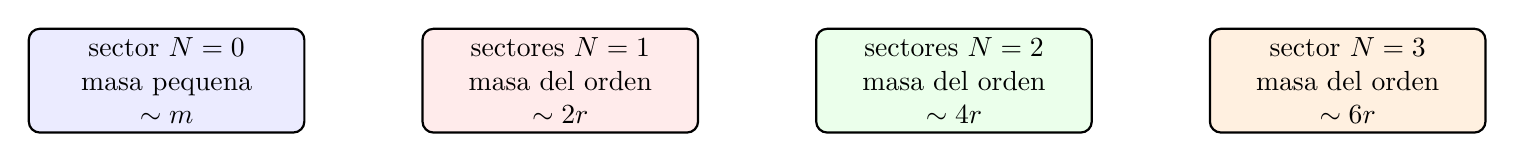
\begin{tikzpicture}[
    box/.style={draw, rounded corners, thick, align=center, minimum width=3.5cm, minimum height=1.2cm}
]
\node[box, fill=blue!8] at (0,0) {sector \(N=0\)\\masa pequena\\\(\sim m\)};
\node[box, fill=red!8] at (5,0) {sectores \(N=1\)\\masa del orden\\\(\sim 2r\)};
\node[box, fill=green!8] at (10,0) {sectores \(N=2\)\\masa del orden\\\(\sim 4r\)};
\node[box, fill=orange!12] at (15,0) {sector \(N=3\)\\masa del orden\\\(\sim 6r\)};
\end{tikzpicture}
\caption{Jerarquia de masas cuando \(\abs{m}\ll 2r\): el sector central queda ligero y los dobladores se apartan energeticamente.}
\end{figure}

\section{La teoria efectiva de baja energia}
Si restringimos la energia a
\begin{equation}
\abs{E}\ll \Delta_{\text{heavy}},
\end{equation}
los sectores con \(N\ge 1\) no se excitan. Entonces la teoria efectiva queda dominada por el sector \(N=0\):
\begin{equation}
H_{\text{low}}(\bm{q})
\simeq
v\sum_{i=1}^3 q_i \alpha_i + m\beta
+
\frac{ra^2}{2}\abs{\bm{q}}^2\beta + \cdots.
\label{c14:eq:lowenergy}
\end{equation}

La primera parte es exactamente el Hamiltoniano de Dirac que queriamos. El siguiente termino es cuadratico en \(\bm{q}\), asi que queda suprimido a energias suficientemente bajas.

\subsection{Que significa \enquote{seleccionar el subsector}}
No significa borrar los otros sectores del Hamiltoniano microscópico. Significa algo mas preciso:
\begin{enumerate}[label=\arabic*.]
    \item existen en la teoria completa;
    \item pero tienen gaps mucho mayores;
    \item por tanto no participan en la dinamica de baja energia;
    \item y el observador infrarrojo solo ve el sector ligero.
\end{enumerate}

Ese es exactamente el sentido correcto de \enquote{emergencia efectiva} en este contexto.

\section{Por que esto esta bien justificado}
Este punto es delicado y merece una justificacion clara.

\subsection{Primer argumento: separacion de escalas}
Si el experimento, simulacion o analisis teorico trabaja con energias \(\abs{E}\ll \Delta_{\text{heavy}}\), no hay energia suficiente para poblar los sectores pesados. Su contribucion queda reducida a correcciones perturbativas.

\subsection{Segundo argumento: estabilidad de la linealizacion}
En el sector central, el termino de Wilson comienza en orden \(q^2\). Por tanto no destruye la estructura lineal tipo Dirac:
\begin{equation}
M(\bm{q}) = m + \frac{ra^2}{2}\abs{\bm{q}}^2+\cdots.
\end{equation}
Esto significa que el limite infrarrojo sigue estando gobernado por el cono relativista.

\subsection{Tercer argumento: compatibilidad con la algebra de Dirac}
El subsector ligero no es un artificio arbitrario, porque sigue estando controlado por las mismas matrices \(\alpha_i\) y \(\beta\) que generan el algebra de Clifford. Eso enlaza directamente con los capitulos donde construimos \(\gamma^\mu\), \(\Sigma^{\mu\nu}\) y la estructura de \(SL(2,\mathbb{C})\).

\section{Que ventanas de parametros son buenas y cuales no}
\subsection{Ventana buena}
La ventana pedagogica mas limpia es
\begin{equation}
r>0,
\qquad
\abs{m}\ll 2r.
\end{equation}
En ella:
\begin{enumerate}[label=\arabic*.]
    \item hay un solo sector ligero;
    \item los demas estan pesados;
    \item la teoria efectiva es Dirac con peque\~na masa \(m\).
\end{enumerate}

\subsection{Ventanas delicadas}
Los puntos
\begin{equation}
m= -2r,\qquad m=-4r,\qquad m=-6r
\end{equation}
son especiales, porque alli uno o mas dobladores adicionales se vuelven tambien ligeros. En esos puntos la seleccion del subsector falla o se vuelve mucho mas sutil.

Por eso, si lo que queremos es un solo sector efectivo controlado, debemos mantenernos lejos de esos valores criticos.

\section{\texorpdfstring{Como se conecta con Weyl y con Dirac \(3+1\)}{Como se conecta con Weyl y con Dirac 3+1}}
Ya podemos ver la pelicula completa.

\subsection{Paso 1: controlar Dirac}
El modelo de Wilson--Dirac nos permite obtener un solo sector de Dirac ligero en \(3D\), mientras los dobladores quedan gappeados.

\subsection{Paso 2: volver al lenguaje covariante}
En ese subsector, las matrices \(\alpha_i\) y \(\beta\) son exactamente las que ya tradujimos al lenguaje covariante mediante
\begin{equation}
\gamma^0=\beta,
\qquad
\gamma^i=\beta\alpha_i.
\end{equation}

\subsection{Paso 3: abrir la puerta a Weyl}
Si luego se introduce una perturbacion que rompa adecuadamente la simetria que mantiene juntos los dos sectores quirales, el cono de Dirac ligero puede desdoblarse en nodos de Weyl controlados. La diferencia es que ahora ese desdoblamiento ocurre dentro de un subsector bien aislado, y no en medio de una nube incontrolada de dobladores equivalentes.

\begin{figure}[h!]
\centering
\begin{tikzpicture}[
    box/.style={draw, rounded corners, thick, align=center, minimum width=3.8cm, minimum height=1.3cm},
    arr/.style={-{Latex[length=3mm]}, thick}
]
\node[box, fill=blue!7] (a) at (0,0) {Wilson--Dirac\\en red};
\node[box, fill=green!7] (b) at (5,0) {un sector Dirac\\ligero};
\node[box, fill=yellow!10] (c) at (10,0) {lenguaje covariante\\\(\gamma^\mu,\Sigma^{\mu\nu}\)};
\node[box, fill=red!7] (d) at (15,0) {posible control\\de sectores Weyl};
\draw[arr] (a) -- (b);
\draw[arr] (b) -- (c);
\draw[arr] (c) -- (d);
\end{tikzpicture}
\caption{Lugar exacto de este paso dentro del programa completo.}
\end{figure}

\section{Lecciones para el proyecto}
Este paso deja seis mensajes importantes.

\subsection*{Mensaje 1}
No basta con encontrar un Hamiltoniano que se parezca localmente a Dirac. Hay que demostrar que los demas dobladores se apartan energeticamente.

\subsection*{Mensaje 2}
El termino de Wilson no se introduce para \enquote{arreglar a mano} la teoria, sino para reorganizar de forma controlada la informacion global de la red.

\subsection*{Mensaje 3}
Seleccionar un subsector efectivo significa trabajar en una ventana de energia donde solo un sector queda dinamicamente accesible.

\subsection*{Mensaje 4}
La condicion \(\abs{m}\ll 2r\) es la forma mas transparente de expresar esa jerarquia de escalas en el modelo pedagogico.

\subsection*{Mensaje 5}
Una vez seleccionado ese subsector, reaparece de forma limpia la estructura de Dirac \(3+1\) que venimos construyendo.

\subsection*{Mensaje 6}
Solo despues de esto tiene pleno sentido volver a preguntar por quiralidad, desdoblamiento Weyl y estructura efectiva de grupos.

\section{Mapa del siguiente paso}
Con este capitulo ya tenemos una respuesta concreta a la pregunta delicada de como aislar un subsector util. El siguiente paso natural es uno de estos dos:
\begin{enumerate}[label=\arabic*.]
    \item introducir una perturbacion concreta que desdoble el sector Dirac ligero en un par de nodos Weyl y seguir la cuenta paso a paso;
    \item estudiar hasta que punto los generadores efectivos derivados antes se realizan de forma aproximada dentro de este subsector aislado.
\end{enumerate}

\section{Resumen final}
El mensaje central de este capitulo es que el problema del doblamiento no se resuelve solo mirando cerca de un nodo: se resuelve organizando toda la estructura global de la red. El modelo de Wilson--Dirac hace eso de manera especialmente clara. Su Hamiltoniano
\[
H(\bm{k})=
\frac{v}{a}\sum_i \sin(k_i a)\alpha_i
+
\left[m+r\sum_i(1-\cos k_i a)\right]\beta
\]
mantiene la estructura tipo Dirac local, pero asigna masas distintas a los diferentes dobladores de la zona de Brillouin.

Cuando \(\abs{m}\ll 2r\), el sector central queda ligero mientras los demas se vuelven pesados. Eso produce exactamente la situacion que necesitabamos: una teoria efectiva relativista bien controlada, incrustada dentro de una dinamica discreta mas grande. Esa es la base correcta para seguir luego con desdoblamientos Weyl, quiralidad y, mas adelante, con la pregunta mas ambiciosa sobre estructura efectiva de simetrias y espacio-tiempo.
